%====|==> ICRC 2019
\subsection{Datos presentados en la ICRC 2019}\label{conjuntoB}

Este conjunto de datos contiene eventos de los tres años posteriores con respecto  a los datos del ICRC 2017. Posteriormente al trabajo \cite{aab2017impact}, la señal de S(1000) fue corregida por las condiciones climáticas en la reconstrucción oficial de eventos. Además el valor de S(1000) estimado para cada evento cambió entre estos dos conjuntos de datos, por parte de la reconstrucción oficial \cite{isabel}. Se realizó también una nueva calibración de la energía mediante eventos híbridos, como la mostrada en la Fig.\,\ref{fig:efd_s38} en el trabajo  \cite{tobepublished}. 

En el conjunto de datos de la ICRC 2019, se realizó los mismos cortes que para el conjunto de A de la sección anterior. En el periodo 2005-2015 de los datos de la ICRC 2019 con los cortes mencionados de energía mayor a $1\,$EeV para eventos verticales, la cantidad de eventos con energías mayores a $1\,$EeV subió de $1\,146\,470$ a  $1\,280\,918$ eventos. %Esto puede deberse a la corrección del clima de los eventos, donde aquellos eventos que estaban por debajo del corte de energía, tras la corrección pudieron estar por encima de este corte. 
Una posibilidad es que la nueva reconstrucción implementada sobre los datos del ICRC 2019, haya aumentado la cantidad de eventos por encima de $1\,$EeV, por eso la energía media bajó de $2.00\,$EeV a $1.91\,$EeV.  Las características de los datos en los rangos de tiempo relevantes se resumen en la Tabla\,\ref{tabla:caracteristicas_ICRC_2019}. 

%====|====|	Tabla de eventos exposure
   \begin{table}[H]
       \centering
       \begin{tabular}{r|c|c|}
    %    {Tiempo }           & {01/01/2005-31/12/2015}   & {01/01/2005-31/12/2018 }\\ \hline 
    \cline{2-3}
                              & \multicolumn{2}{c|}{ICRC 2019} \\ \cline{2-3}
         Inicio:              & 01/01/2005      & 01/01/2005\\
         Fin:                 & 31/12/2015      & 31/12/2018\\  
         Número de eventos:   &  $1\,280\,918$     			    &  1635045     		        \\ 
         Energía media:       &  1.91				        &	1.92				        \\ 
         Corte en energía:    &  $>1$ EeV       		 	    &  $>1$  EeV       		 \\ 
         Corte en ángulo cenital:	&  $\theta<60^o$ 				    & $\theta < 60^o$\\ \cline{2-3}
       \end{tabular}
       \caption{Características de los datos de la ICRC 2019 utilizados para los ajustes de esta sección.} \label{tabla:caracteristicas_ICRC_2019}
   \end{table}

   En la Fig.\,\ref{fig:rate_new_18} se muestran las tasas de eventos por día para energía mayores a $1\,$EeV y $2\,$EeV, con la energía corregida por los efectos climáticos según la reconstrucción oficial \cite{data}.  Comparemos las tasas de eventos por hora del día de los eventos, por encima de $1\,$EeV y $2\,$EeV con las tasas para el conjunto  A. Por encima de $1\,$EeV, se aprecia un remanente de la modulación del clima diaria comparado con la tasa para $2\,$EeV. Esto se debe a que el arreglo principal tiene eficiencia completas para energías mayores a $3\,$EeV, comentado anteriormente. Por encima de 2\,EeV, la modulación en la tasa ya no es apreciable. 


   Existe una modulación remanente en la tasa de eventos con energía mayor a 1 EeV como se aprecia en la Fig.\,\ref{fig:rate_new_18} y \ref{fig:rate_new_18_2EeV}. Esto se debe que la señal es mayor que la esperada como consecuencia de las condiciones atmosféricas en el momento del evento, por lo tanto la eficiencia del disparo ante este evento también es mayor. De esta forma la eficiencia tiene una dependencia con las condiciones atmosféricas.
%====|====|	2005-2019	rate day over 1 EeV
%====|====|	2005-2019	rate hour of the day	1 EeV
   \begin{figure}[H]
       \centering
      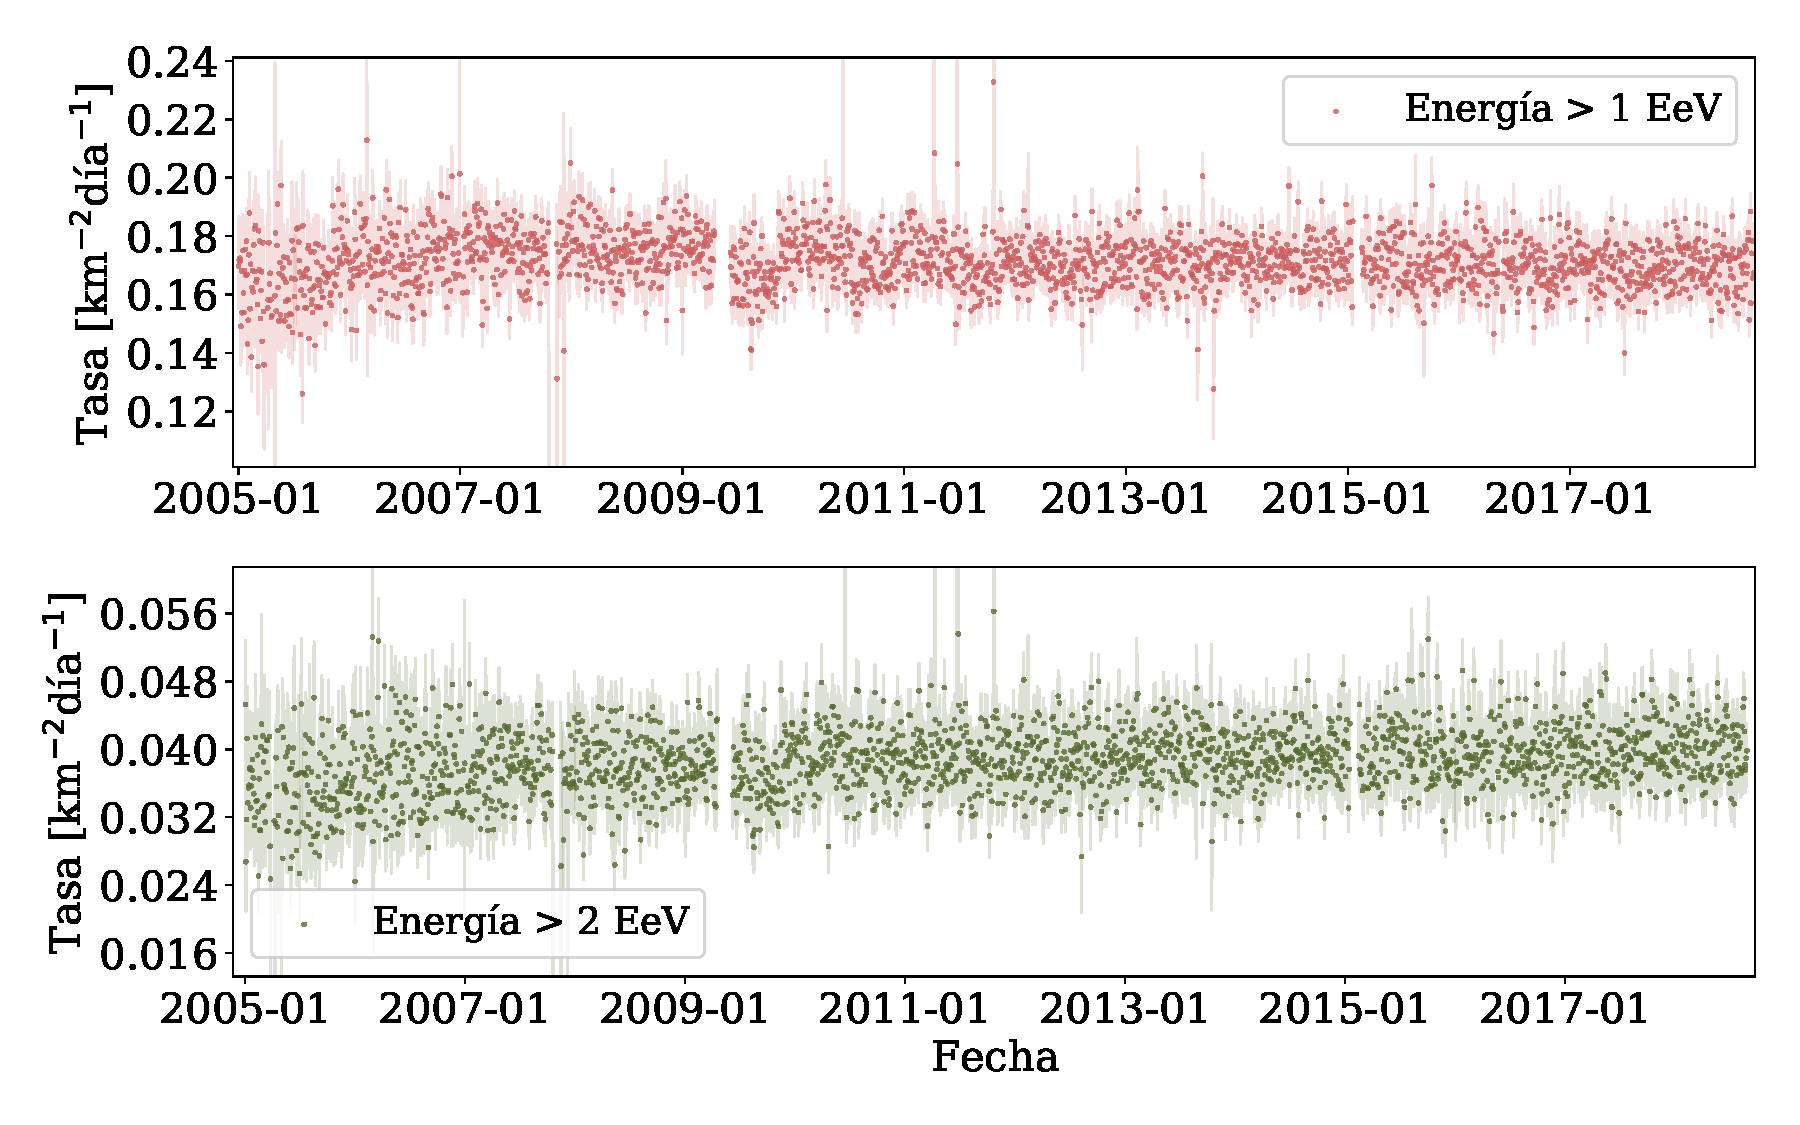
\includegraphics[width=0.8\textwidth]{Graphs/rate_dayly/herald_above_1EeV_2EeV_rate_day.pdf}
       \caption{Tasa de eventos promedio por cada día desde inicios del 2005 hasta inicios del 2018 del conjunto de datos presentado en la ICRC 2019. Se muestran las tasas para dos cortes en energía, mayor a $1\,$EeV y mayor a $2\,$EeV}\label{fig:rate_new_18}
   \end{figure}



   \begin{figure}[H]
       \centering
      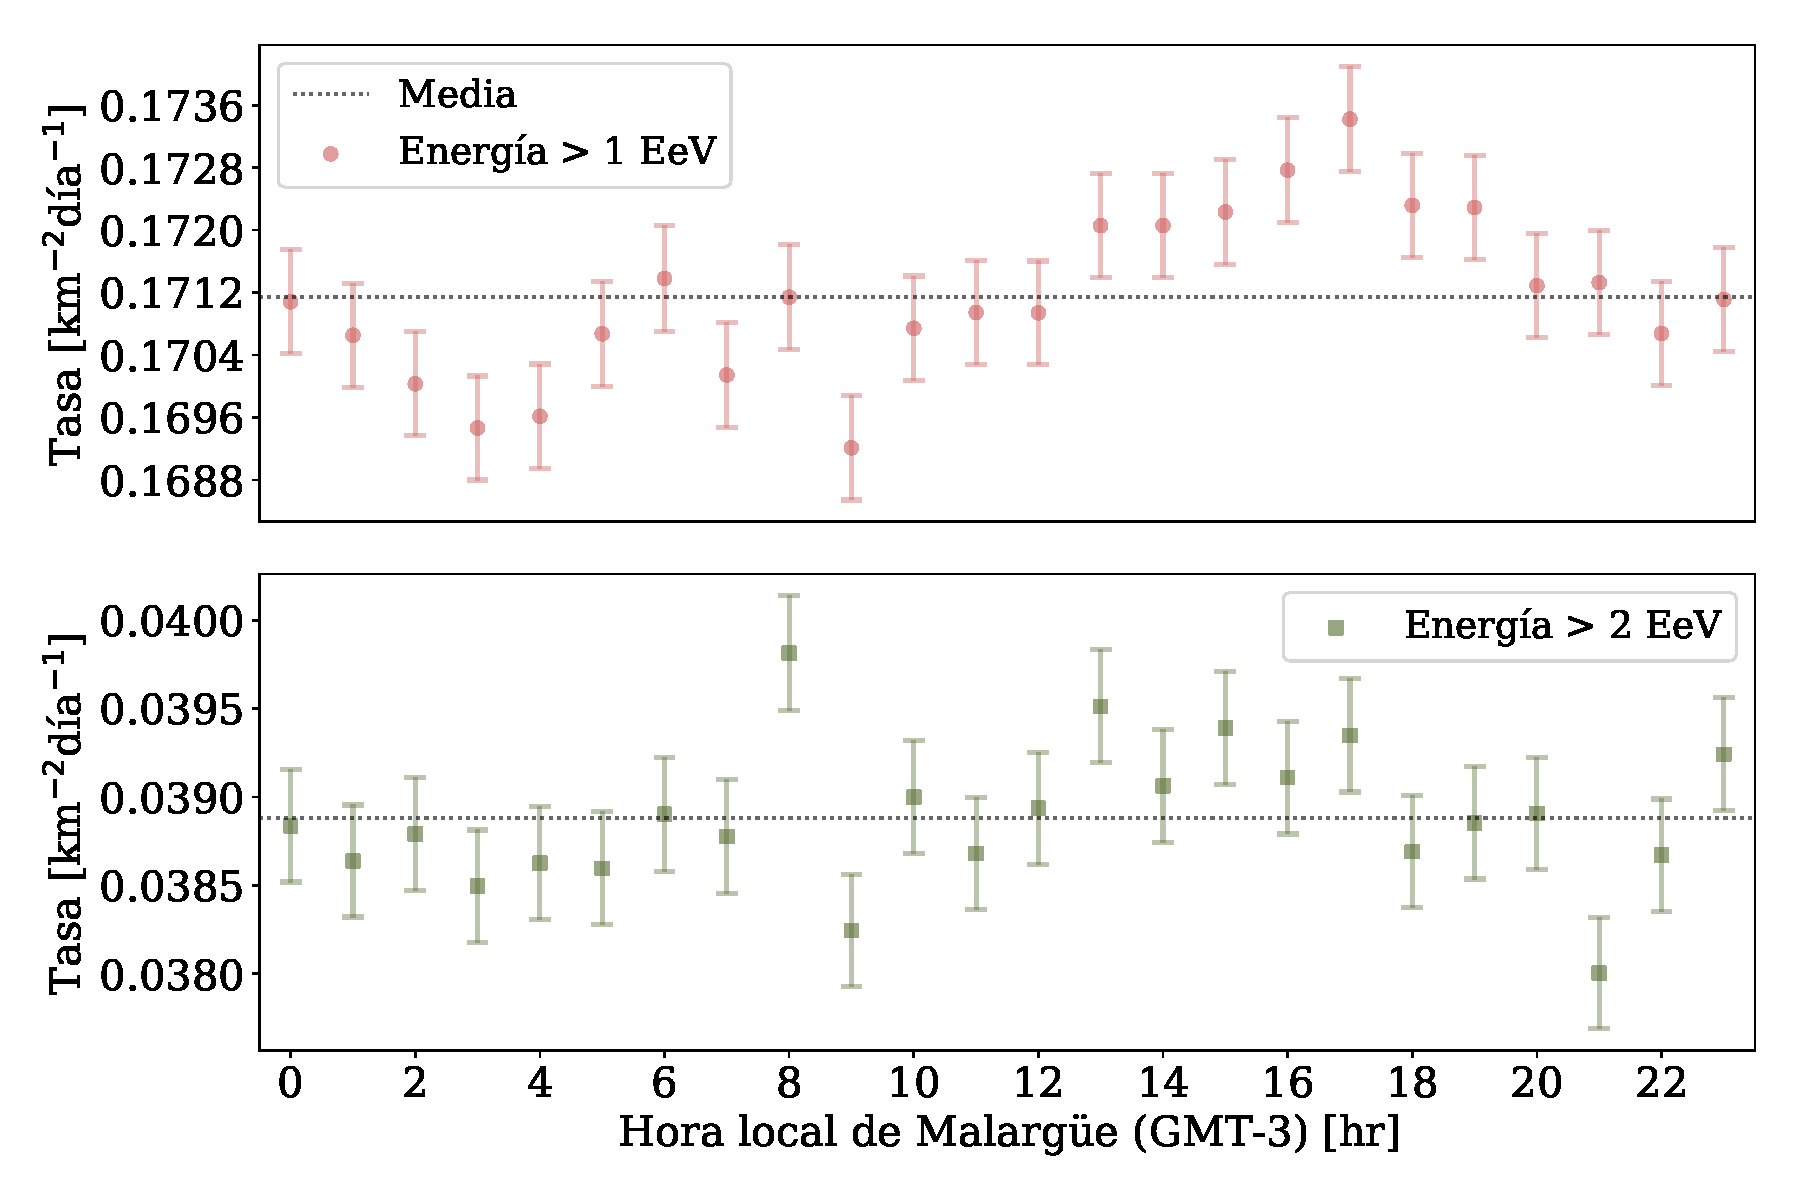
\includegraphics[width=0.8\textwidth]{Graphs/rate_hour_of_the_day/herald_above_1EeV_and_2EeV_hour_of_the_day.pdf}
       \caption{Tasas de eventos  por hora del día por unidad de área desde inicios del 2005 hasta inicios del 2018 del conjunto de datos presentado en la ICRC 2019.  Se muestran las tasas para dos cortes en energía, mayor a $1\,$EeV y mayor a $2\,$EeV}\label{fig:rate_new_18_2EeV}
   \end{figure}


%====|==>ICRC 2019 S$_{38}$-Sin Corrección
\subsection{Datos presentados en la ICRC 2019 usando $S_{38}$ sin corregir por el clima} \label{sin_corregir_s38}


Además de tener más estadística de los eventos registrados, durante el periodo 2016-2018 también se recabaron datos sobre el clima en el observatorio. En la modulación del clima estudiada con el conjunto A, se  realiza un corte de la energía sin corregir. En esta sección se realiza el análisis de la modulación mediante un  corte sobre la señal medida por el arreglo principal. En el conjunto de datos de la ICRC 2019, es posible acceder al valor de S(1000) sin corregir por el trabajo \cite{aab2017impact}, por lo que uno puede obtener el valor de S$_{38}$ sin corregir mediante la expresión
\begin{equation}
S_{38} = \frac{S(1000)}{S(1000)_w}S_{38,w}
\label{eq:s38_w}
\end{equation}
donde las variables $S(1000)_w$ y $S_{38,w}$ indican los valores corregidos por clima. Estas variables están listadas en el conjunto de datos presentado en la ICRC 2019. 

Dado que los trabajos anteriores se basaron en la energía para hacer el corte de los eventos, se realizó el corte con la señal de $S_{38}\ge 5.37\,$VEM correspondiente a 1\,EeV aproximadamente. Las características de este conjunto de datos están resumidos en la Tabla\,\ref{tabla:caracteristicas_ICRC_2019_S38}.
%====|====|	Tabla de eventos exposure
   \begin{table}[H]
       \centering
       \begin{tabular}{r|c|c|}
    %    {Tiempo}                & {01/01/2005-31/12/2015}   & {01/01/2005-31/12/2018 }\\ \hline
    \cline{2-3}
                              & \multicolumn{2}{c|}{ICRC 2019} \\ \cline{2-3}
 
       Inicio:                 & 01/01/2005                 &  01/01/2005 \\
       Fin:                    & 31/12/2015                 &   31/12/2018 \\
       Número de eventos:       &   $1\,267\,265$     	    &  $1\,618\,717$     		\\ 
       Energía media:           &  1.89        		 	    &  1.90        		\\  
       Corte en S$_{38}$: 	   &  $>5.37$\,VEM   		 	    &  $>5.37$\,VEM       	\\  
       Corte en ángulo cenital: &  $\theta<60^o$ 			 	 & $\theta<60^o$\\ \cline{2-3}
       \end{tabular}
       \caption{Características de los datos de la ICRC 2019 con el corte en la señal de S$_{38}$ utilizados para los ajustes de esta sección.} \label{tabla:caracteristicas_ICRC_2019_S38}
   \end{table}
   
%====|====| Tabla del fit
   Con estos eventos, se realizó un  ajuste de los parámetros del clima para todos los ángulos cenitales de la tasa de eventos por hora, así se obtienen los coeficientes promediados por ángulo cenital. Estos parámetros son presentados en la Tabla\,\ref{tabla:parametros_ICRC_2019_S38}. Se observa que para ambos periodos estudiados los parámetros obtenidos son compatibles entre sí, además de ser compatibles con los resultados obtenidos para el periodo 2005-2015 de los datos de la ICRC 2017 y los parámetros de \cite{aab2017impact} presentados en la Tabla\,\ref{tabla:parametros_ICRC_2017}.

   \begin{table}[H]
       \centering
       \begin{tabular}{c|c|c}
       {Parámetro}                 & {2005-2015}    		        & {2005-2018}    \\ \hline \hline
       $a_P$ [hPa$^{-1}$]          & $ (-3.3\pm 0.3)\times 10^{-3}$& $(-3.2\pm 0.2)\times 10^{-3}$  \\ \hline
       $a_\rho$ [kg$^{-1}$m$^3$]   & $ -1.75\pm 0.04$            	& $ -1.71\pm 0.03$       \\ \hline
       $b_\rho$ [kg$^{-1}$m$^3$]   & $ -0.51\pm 0.04$             	& $ -0.52\pm 0.03$       \\ \hline
       $\chi^2_\nu$                & $1.00616$                     & $1.01819$              \\   
       \end{tabular} 
       \caption{Parámetros del clima obtenidos para todos los ángulos cenitales para los dos rangos de tiempo estudiados de los datos de la ICRC 2019 con el corte en la señal de S$_{38}$.} \label{tabla:parametros_ICRC_2019_S38}
   \end{table}
   
   Calculando la tasa de eventos esperado con los parámetros de la Tabla\,\ref{tabla:parametros_ICRC_2019_S38}, esta se comparan con la tasa experimental medida con el arreglo principal, que se muestra en la Fig. \ref{fig:rate_new_18_S38} para el rango de tiempo 2005-2018. En estos gráficos se observa que la modulación del clima tiene las mismas características que las observadas en la sección \ref{icrc2015} salvo un aumento en la tasa media de eventos.

   \begin{figure}[H]
    \centering
       \begin{subfigure}[b]{0.85\textwidth}
       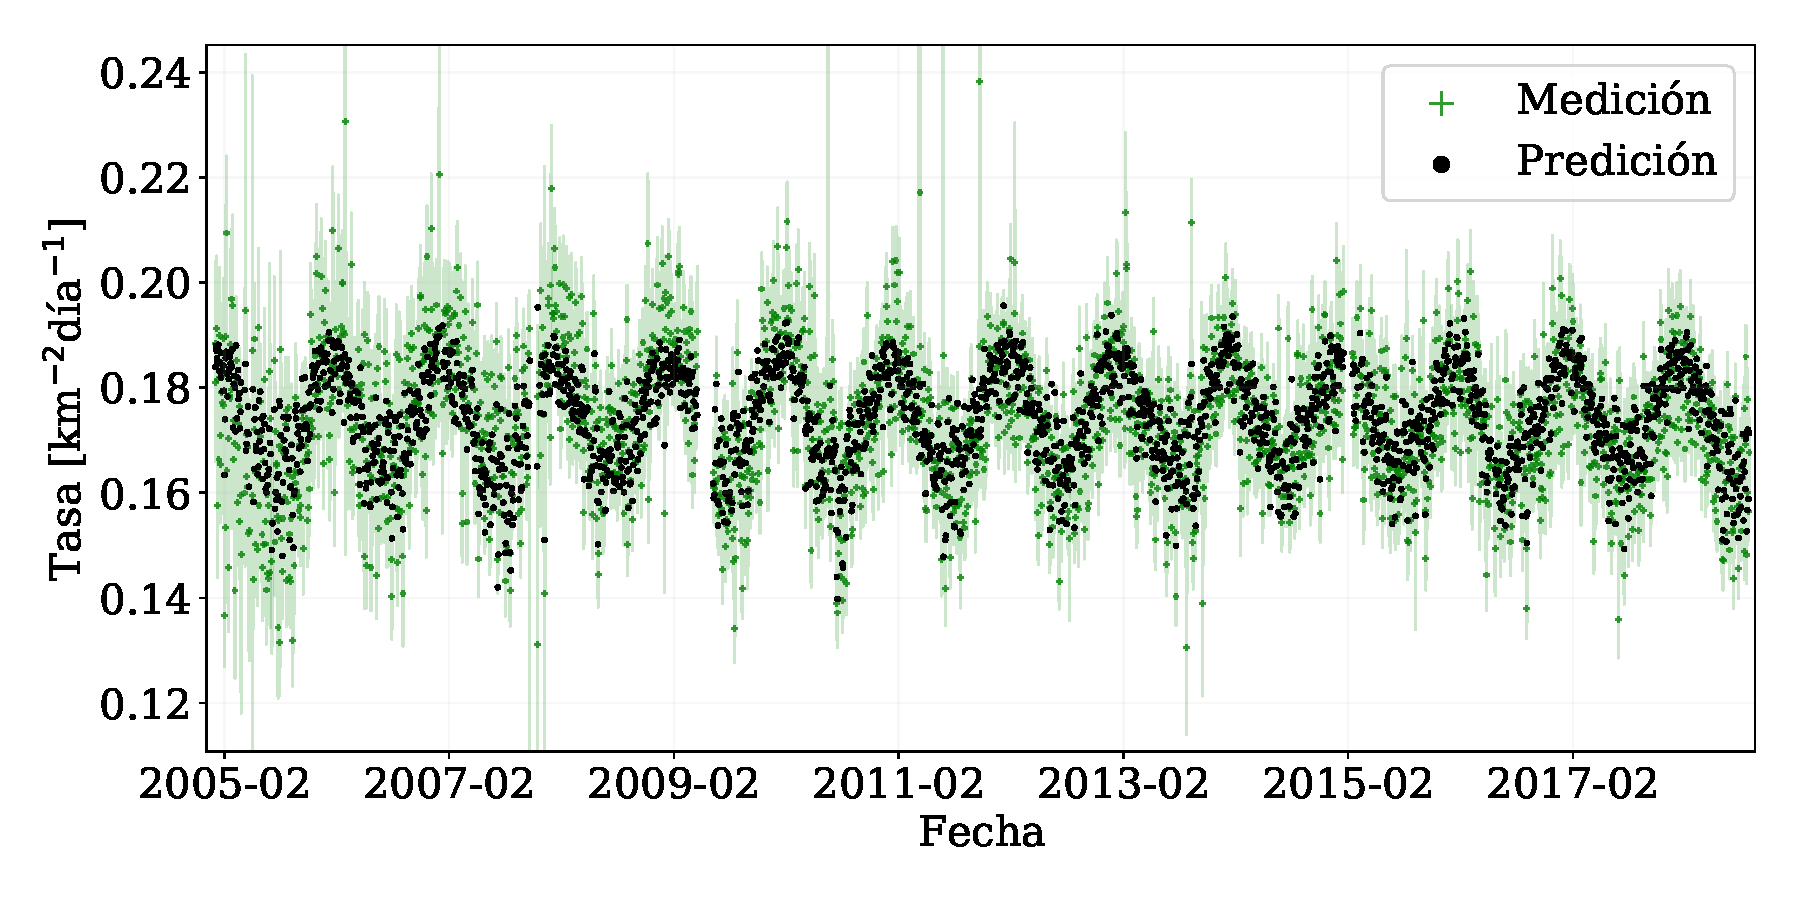
\includegraphics[width=\textwidth]{Graphs/rate_dayly/0EeV_ICRC_2019_S38_05_18.pdf}
       \caption{Tasa eventos por cada día por unidad de área}
       \label{fig:rate_day_ICRC_19_S38_05_18}
       \end{subfigure}\\%
    %    \hspace{\fill}
       \begin{subfigure}[b]{0.85\textwidth}
       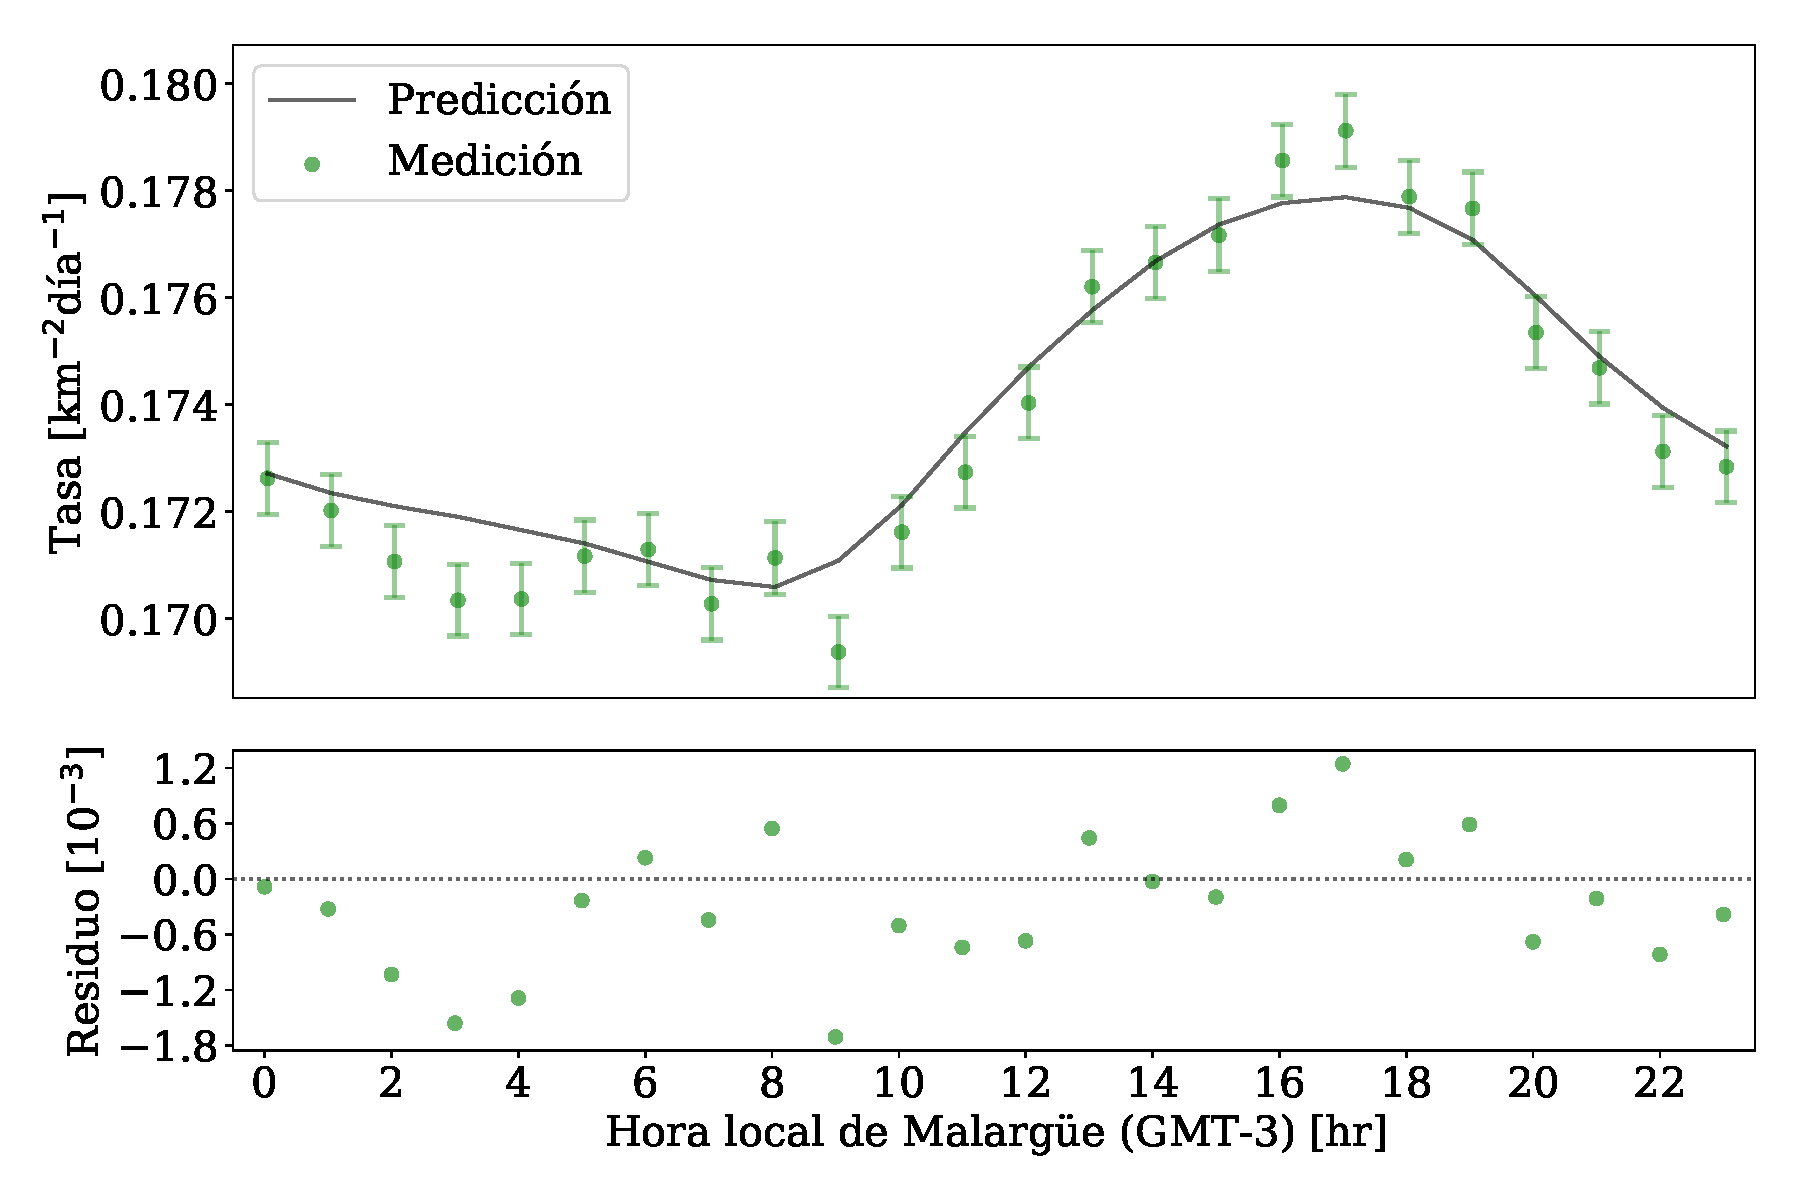
\includegraphics[width=\textwidth]{Graphs/rate_hour_of_the_day/S38_above_0EeV_hour_of_the_day.pdf}
       \caption{Tasa de eventos promedio por hora del día}
       \label{fig:rate_2015_ICRC_19_S38_05_18}
       \end{subfigure}%
       \caption{Tasa de eventos desde inicios del 2005 hasta inicios del 2018 de los datos de la ICRC 2019 con el corte en la señal de S$_{38}$. La predicción es obtenida por los parámetros calculados en este trabajo.}\label{fig:rate_new_18_S38}
   \end{figure}

%====|====|	Weather params
\subsubsection{Ajuste de los parámetros del clima}

En esta sección se clasificó los eventos mediante el valor de $sin^2\theta$ y se realizó el ajuste para obtener los parámetros del clima. Este ajuste se realizó en el periodo 2005-2018. Los valores obtenidos se resumen en la Tabla\,\ref{tabla:cuadratica_ICRC_2019_S38} y se  observan en la Fig.\,\ref{fig:parameters_new_S38}. Comparando estos resultados con los resultados de \cite{aab2017impact}, los eventos mediante el valor S$_{38}$  conservan la tendencia con $sin^2\theta$ que se observa en los datos de la ICRC 2017 en la Fig.\,\ref{fig:parameters_old}. Además los parámetros obtenidos mediante el corte por S$_{38}$ son comparables con los resultados obtenidos para el conjunto de datos de la ICRC 2017. Por lo que puede decirse que la modulación del clima es apreciable  hasta el día de hoy con una amplitud comparable al año 2015.

%====|====|====| ap, arho, brho 2005-2015  2005-2019 vs JINST over 1 EeV
       \begin{figure}[H]
        \centering
           \begin{subfigure}[b]{0.73\textwidth}
           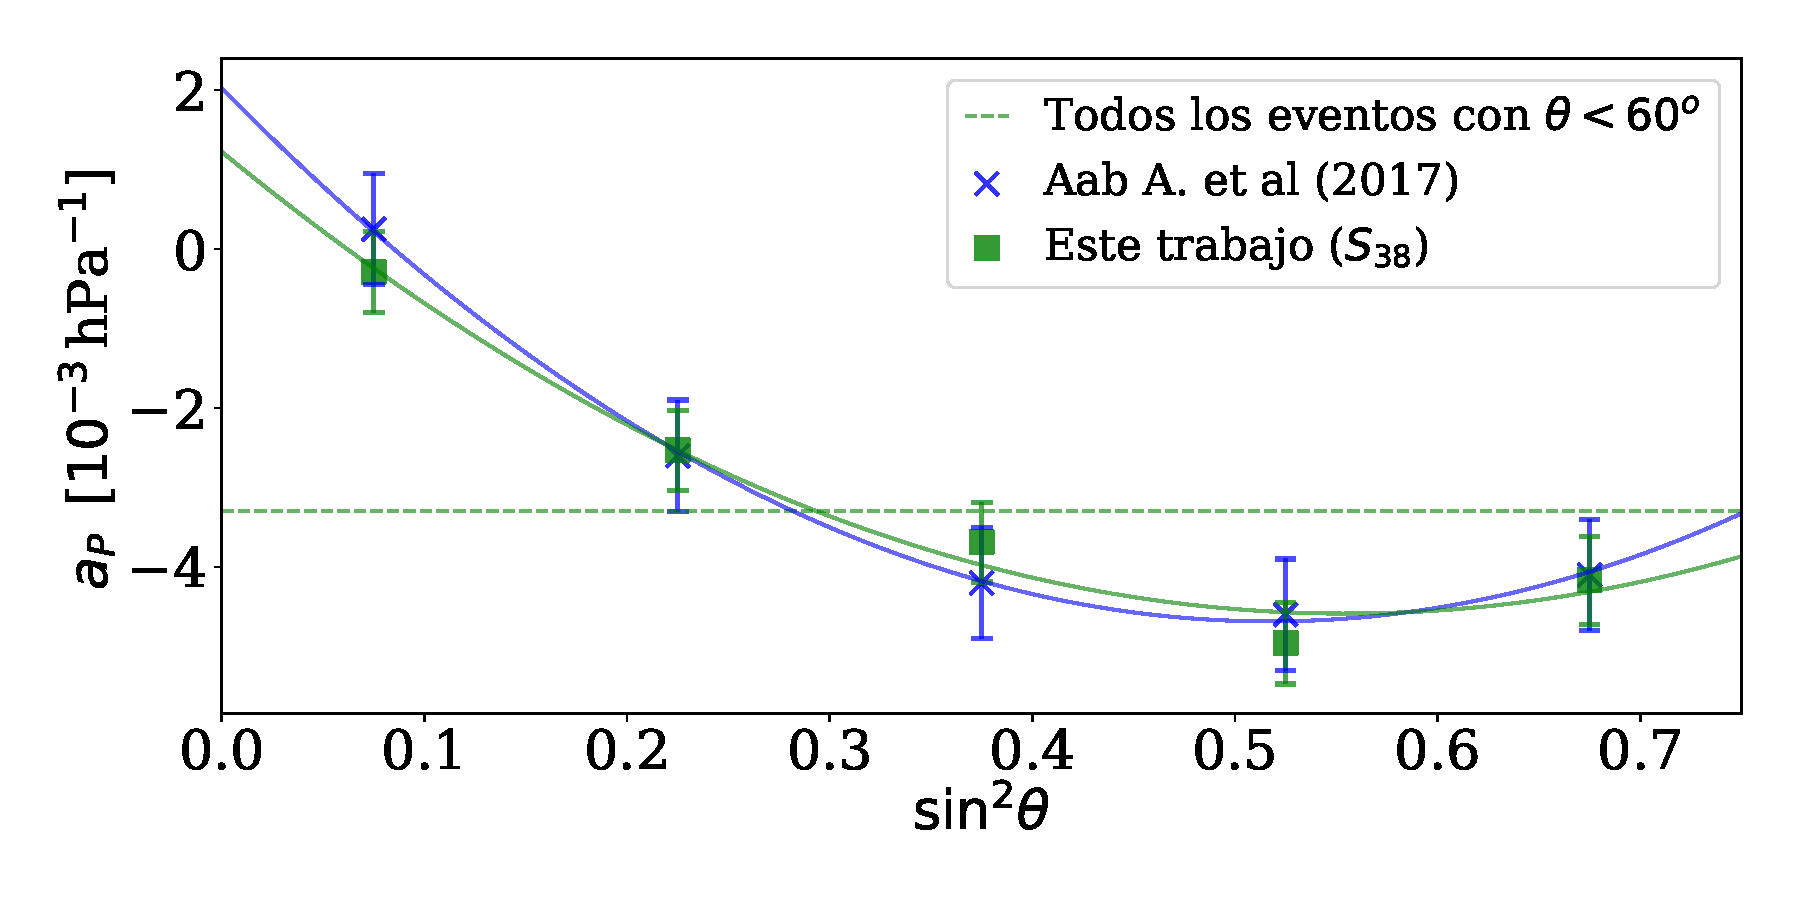
\includegraphics[width=\linewidth]{Graphs/params/ap_ICRC_2019_S38_above_0EeV.pdf}
           \caption{Parámetro $a_P$ }
           \label{fig:ap_2019_S38}
           \end{subfigure}\\%
        %    \hspace{\fill}
           \begin{subfigure}[b]{0.73\textwidth}
           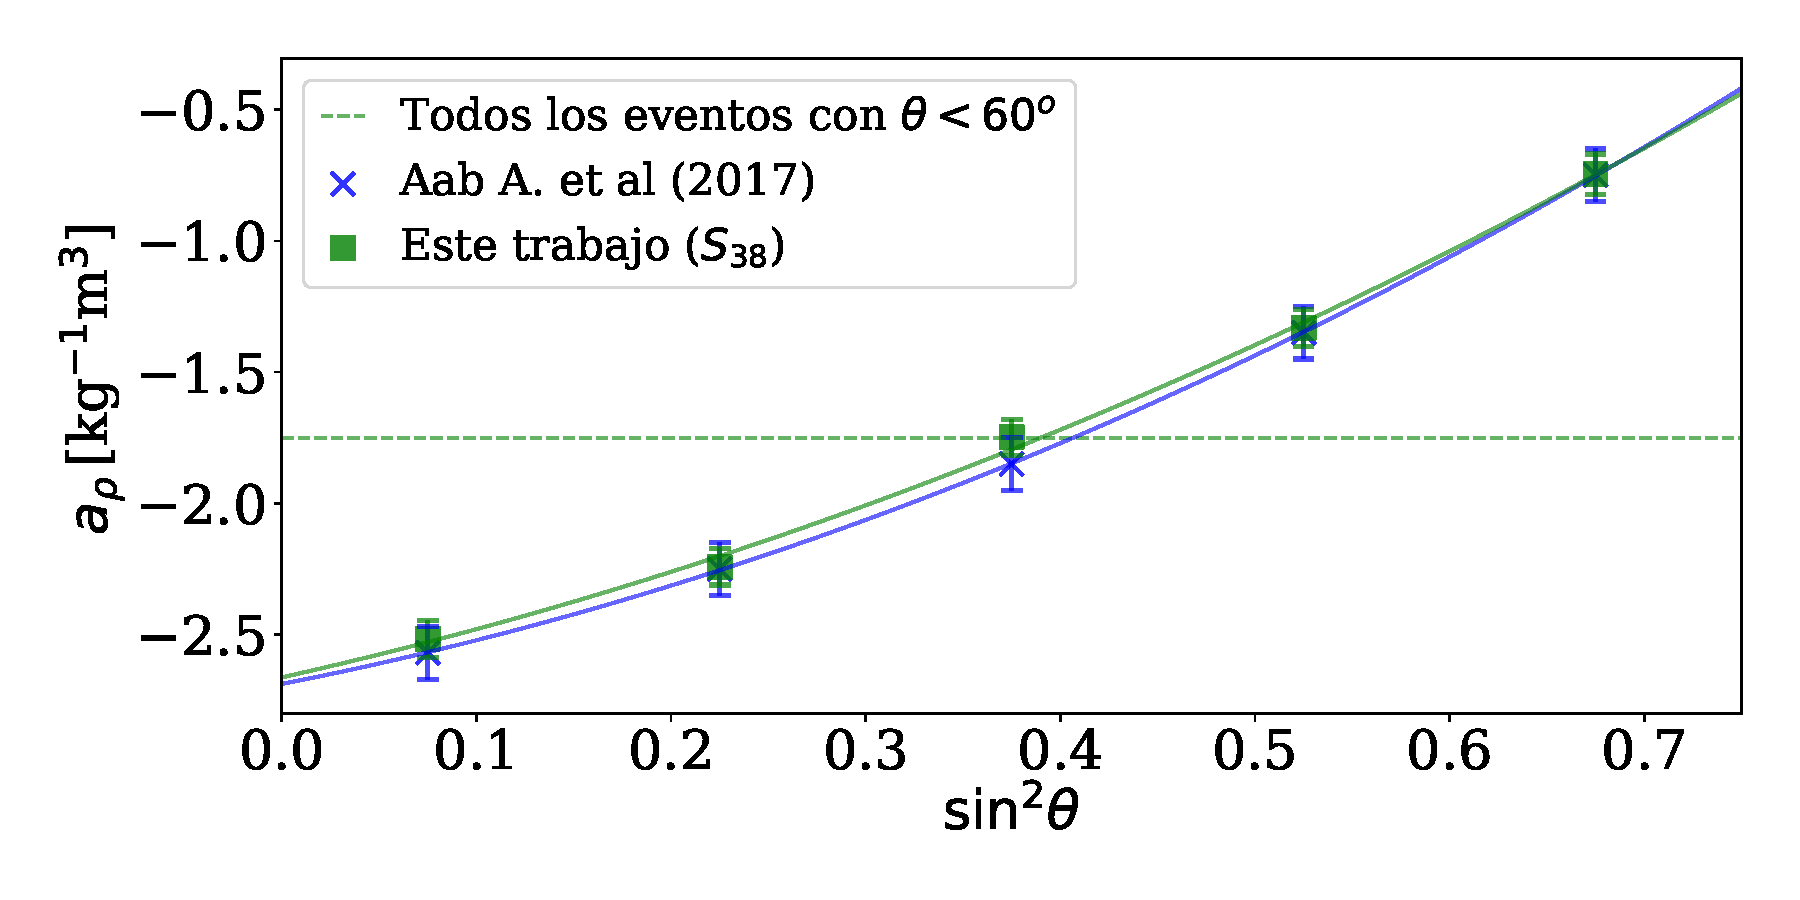
\includegraphics[width=\linewidth]{Graphs/params/arho_ICRC_2019_S38_above_0EeV.pdf}
           \caption{Parámetro $a_{\rho}$ }
           \label{fig:arho_2019_S38}
           \end{subfigure}\\%
        %    \hspace{\fill}
           \begin{subfigure}[b]{\textwidth}
           \centering
           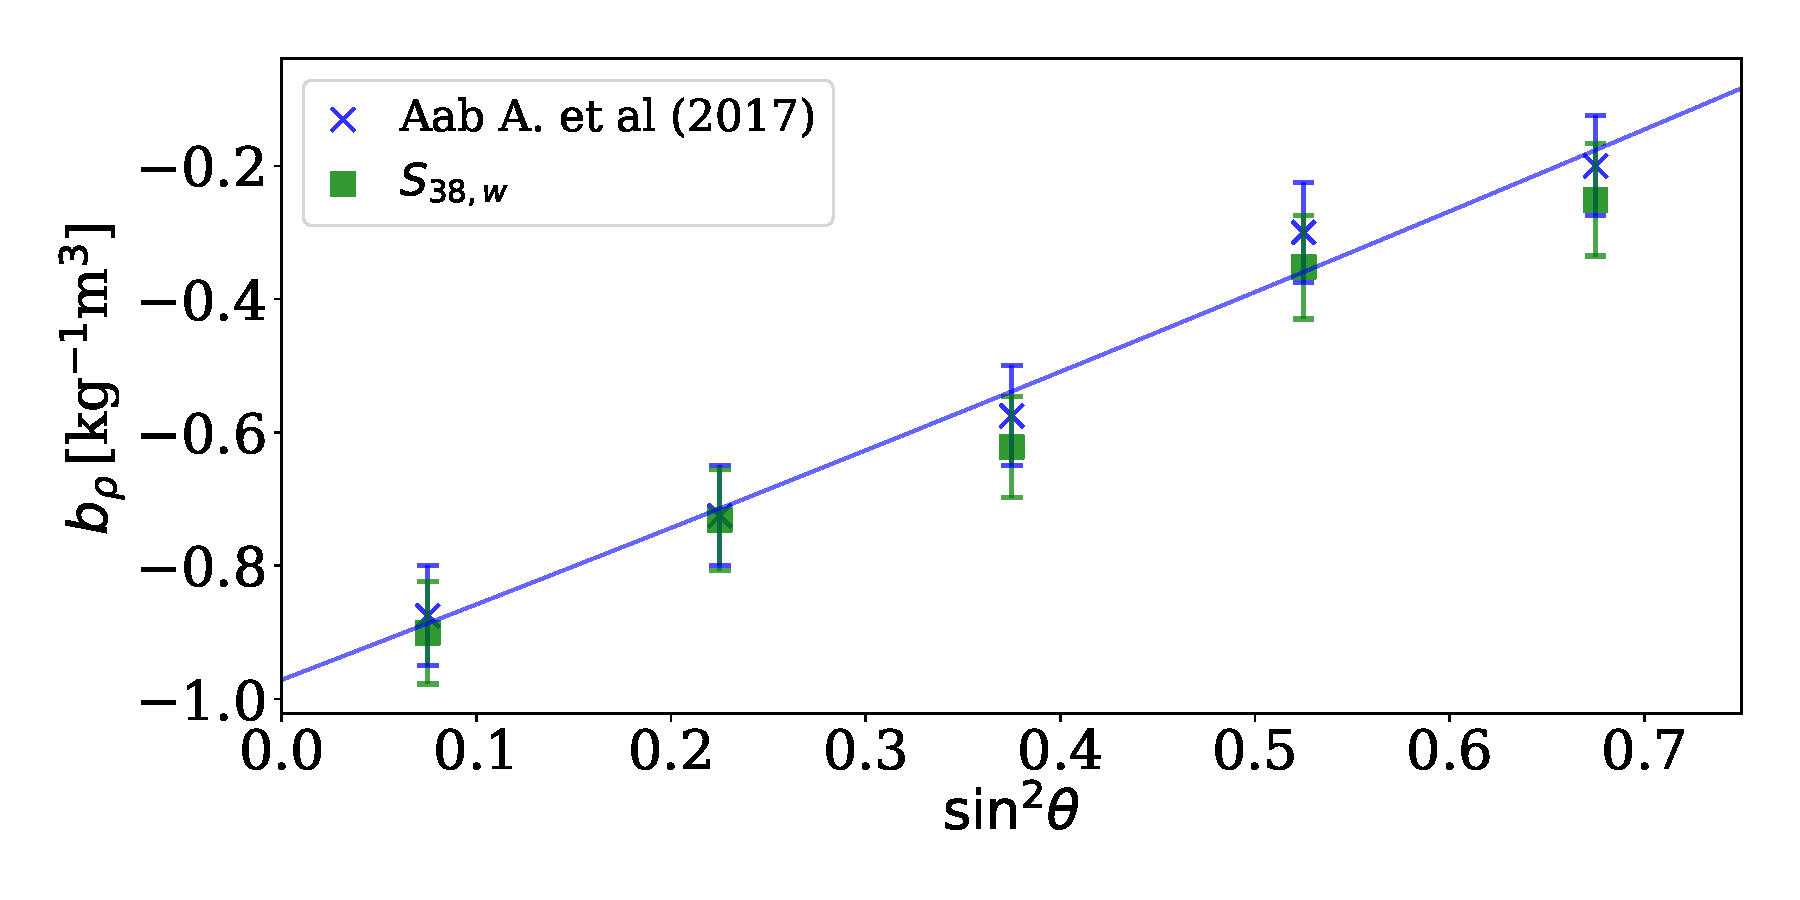
\includegraphics[width=0.73\linewidth]{Graphs/params/brho_ICRC_2019_S38_above_0EeV.pdf}
           \caption{Parámetro  $b_{\rho}$	 }
           \label{fig:brho_2019_S38}
           \end{subfigure}%
           \caption{Parámetros de la modulación del clima considerando los datos sin corregir con el clima y la reconstrucción anterior.}\label{fig:parameters_new_S38}
       \end{figure}
%====|====|====| Tabla de c0, c1, c2
           \begin{table}[H]
               \centering
               \begin{tabular}{l|l|l|l}
                {Parámetros}						        & {Coeficiente}	    & {Este Trabajo} & Reportado por { \cite{aab2017impact}}	\\ \hline \hline
                \multirow{3}{*}{$a_P$ [hPa$^{-1}$]}  		&  $c_0$				& $ (0.12\pm0.05)\times 10^{-3}$	    & $(2.1 \pm 0.09)\times 10^{-3} $	\\ \cline{2-4} %Done
                                                           &  $c_1$				& $ (-2.0\pm0.3)\times 10^{-3}$		& $(-2.6  \pm 0.6)\times 10^{-3} $	\\ \cline{2-4} 
                                                           &  $c_2$				& $ (1.9\pm0.4)\times 10^{-3}$		& $(2.6   \pm 0.7)\times 10^{-3} $	\\ \hline \hline% 
               
                \multirow{3}{*}{$a_\rho$ [kg$^{-1}$m$^3$]} &  $c_0$			& $-2.66   \pm 0.07$	& $ -2.7  \pm 0.1  $\\ \cline{2-4} 
                                                            &  $c_1$			& $ 1.7    \pm 0.4 $	& $ 1.5   \pm 0.8  $\\ \cline{2-4} 
                                                           &  $c_2$			& $ 1.7    \pm 0.6 $	& $ 2.2   \pm 1.0  $\\ \hline \hline %
               
               \multirow{3}{*}{$b_\rho$ [kg$^{-1}$m$^3$]} 	&  $c_0$			& $-0.98    \pm 0.08$	& $-1.0   \pm 0.1 $	\\ \cline{2-4} 
                                                           &  $c_1$			& $ 1.00    \pm 0.5$	& $ 1.2   \pm 0.8  $	\\ \cline{2-4} 
                                                           &  $c_2$			& $ 0.1    \pm 0.6$		& $ 0.0   \pm 1.1  $	\\ \hline  \hline
               
               \end{tabular}	
               \caption{Tabla de los coeficientes obtenidos con el S$_{38}$ sin corregir por el clima, comparados con el trabajo anterior} \label{tabla:cuadratica_ICRC_2019_S38}
           \end{table}

%=================================================================================
%=================================================================================
%=================================================================================
%=================================================================================


%====|==>ICRC 2019 Reconstrucción con este trabajo
\subsection{Datos presentados en la ICRC 2019 usando la energía reconstruída en este trabajo}

Se realizó la corrección del valor de S$_{38}$ con los parámetros del clima presentados en la Tabla.\,\ref{tabla:cuadratica_ICRC_2019_S38} sobre el conjunto de datos de la ICRC 2019. Con este valor corregido se calculó la energía corregida mediante la Ec.\,\ref{eq:s38_energy}. Para una energía mayor de $2\,$EeV, se espera que los efectos del clima sean despreciables tras la corrección, porque se acerca a la eficiencia máxima de los detectores de superficie. %El método de CIC está determinado usando los eventos donde el arreglo principal tiene un eficiencia máxima, evitando la susceptibilidad del disparo de los detectores.

En la Fig.\,\ref{final} se comparan las tasas de eventos por hora del día para el conjunto de datos de la ICRC 2019 y para la corrección de energía realizada en este trabajo. En la figura superior se muestra la tasa de eventos por hora del día del conjunto de datos de la sección \ref{conjuntoB}, comparada con la tasa de eventos para la energía corregida por este trabajo, presentada en la figura inferior. En ambos casos, la tasa tras la corrección queda plana, siendo despreciable el error sistemático de la modulación del clima.

Cabe aclarar que para la corrección de la energía para este trabajo, no se consideraron las posibles modulaciones de los valores del CIC o del posible cambio en los coeficientes de la Ec.\ref{eq:s38_energy}, debido a que estos coeficientes son calibrados con eventos híbridos, la señal corregida puede variar estos coeficientes.


